\chapter{Gap Reconstruction}
One of the more common problems in citizen science projects is gaps in data. This can happen either if the network connection is unstable or the test equipment gets prematurely turn off. This can greatly degrade the data quality, and lead to errors in the application. One way to deal with this problem is do use mathematical gap filling techniques to come with a qualified guess on how the data would look like in the gap. 

In order to use this methods we must assume that the missing data in the gap follows the same behaviour as the data on each side off the gap. Is the signal so stochastic that this is not the case gap filling is not recommended\citep{RefWorks:10}. 

In the case of the SmartHG project the data can be seen to have a part that is dependency on the previous and future data plus a stochastic part that are determined by the user and the appliance. Due to the stochastic part a perfect reconstruction is not possible, but it is the hypotheses that the non stochastic part is still so dominant that a decent reconstruction is possible. 
\section{Gaps In SmartHG Dataset}
The gaps in the SmartHG project dataset is caused by a lot of different sources. This makes the type of gaps different from case to case. Three aspects of a gap is important for the gap filling: The size of the gap, the data known before the gap, and the data known after the gap. 
\subsection{Gap Size}
Looking at the different gaps in the dataset we see that the normal gap is relatively small. This can be seen on figure \ref{fig:GapSize}
\begin{figure}[H]
\centering
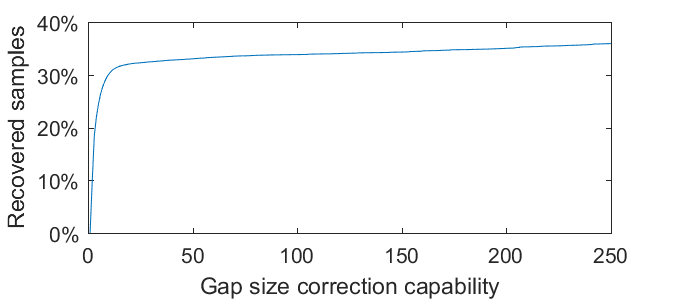
\includegraphics[width=0.8\textwidth]{billeder/CorrectionCapability.png}
\caption{Gap size}
\label{fig:GapSize}
\end{figure}
This is good since the signal part stochastic. The grater the gap, the greater influence does the stochastic part have on the signal. Smaller gaps can therefore be fixed with greater success. 
\subsection{Past And Future Availability}
It is also important how many samples are available on the left and right side of the gap. If there is a lot of gaps in the signal it can create a scenario where there only is a small amount of good data between the gaps. This makes it hard to reconstruct the data, since there is very few points to extract information about the region. 
\begin{figure}[H]
\centering
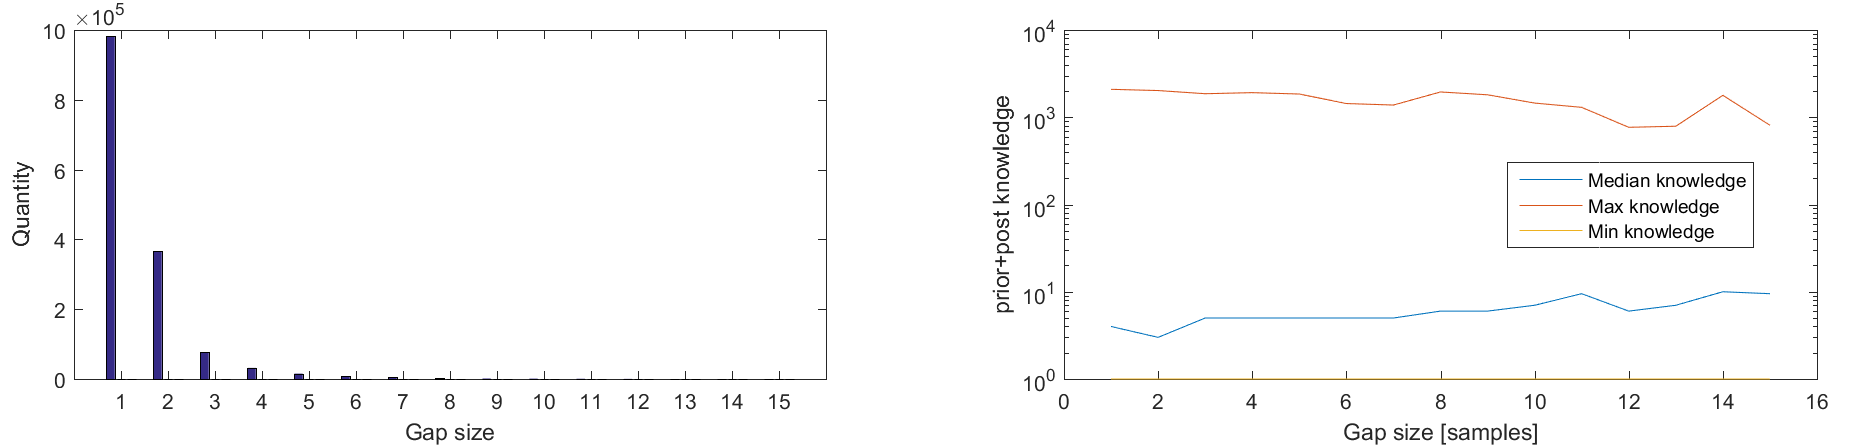
\includegraphics[width=1\textwidth]{billeder/GapInfo.png}
\caption{Past and future availability}
\label{fig:PAF}
\end{figure}
As seen on figure \ref{fig:PAF} \fxnote{Write something more when you know the result}

\section{Gap Filling Methods}
Various methods exists for gap filling. Five popular algorithms have been implemented and validated on the SmartHG project data.

\subsection{Papoulis-Gerchberg Algorithm}
\label{T:PGA}
The Papoulis-Gerchberg algorithm is a multi gap filling algorithm, meaning it is capable of correcting more than one gap at the time. This makes the algorithm preform good in conditions with many gaps and few available data points between the gaps, since it can collect information about the signal from multiple fragments signal \citep{RefWorks:11}. The Papoulis-Gerchberg algorithm works under the assumption that the signal is a periodic stationary signal whit a known bandwidth. The signal will therefore consist of $M$ frequency components, and everything outside the band is assumed to be noise. The signals in the SmartHG is not stationary, but for small snippets can approximately stationariness be assumed. 

The true bandwidth is also unknown in the signal. The Papoulis-Gerchberg algorithm is very depended on the bandwidth for a correct reconstruction. A modified version of the algorithm that estimates the bandwidth, by varying the frequency components $M$ and analysing the mean square error on the known signal is therefore used \cite{RefWorks:13}. This approach has fairly good at estimating the true value of $M$, but it is time-consuming.

\subsection{Wiener Filling Algorithm}
The Wiener filling algorithm is a extension of a Wiener predictor. Like the Wiener predictor it assumes that there exist a linear relationship between the next sample and the previous samples. By trying to predict the missing samples from both sides of the gap, and combining the knowledge it estimates the missing samples \citep{RefWorks:14}. For larger gaps does this methods rely on earlier predictions to close the gaps. This result in errors being accumulated over the gaps. The method is fast, and is therefore suited for large data with small gaps. 

\subsection{Spatio-Temporal Filling Algorithm}
The Spatio-Temporal filling algorithm uses singular spectrum analysis to split the signal into a series of sub-signals. The sum of the sub-signals are the original signal, and the sub-signals is ordered so the most dominant is first, and the least dominant is last. 

The reconstruction philosophy is that the gap has introduced noise in the signal, but a sum of only the most dominant sub-signals must be close to the original signal without noise. But in order to know how many sub-signals to include in this sum, we introduce a other artificial gap. While the sub-signals are being accumulated the mean square error of the artificial gap is observed, when this hits its peek it is assumed that the reconstruction is as good as possible \cite{RefWorks:15}.

This method is very popular for gap filling. It has shown to be very noise resistant since it finds the overall trends in the data. It does require quite a lot of data to be known post and prior to the gap, since a artificial gap must be introduced. Since it is based on singular spectrum analysis it assumes that the signal consist of stationary processes, like the Papoulis-Gerchberg Algorithm in section \ref{T:PGA}.

\subsection{Envelope Filling Algorithm}
\label{T:EGA}
Unlike the previous described methods does the Envelope filling algorithm not depend on frequency analyses, but rather on the expected power of the signal. Bye looking at the envelope of the signal it assumes that all local maxima and minima must lie on the  upper and lower envelope. It then looks at the data prior and post the gap and try to estimate the number of local maxima and minima in the gap, and their locations. It does this by looking for patterns in the time series data \citep{RefWorks:6}. When the new maxima and minima is found the points is connected by using spline \cite{RefWorks:16}. 

The methods does not make any assumptions about the signals stationariness or bandwidth. The method can also be used on none equally spaced time series. 

\subsection{Empirical Mode Decomposition Filling Algorithm}
The empirical mode decomposition filling algorithm uses empirical mode decomposition, to break the signal in to intrinsic mode functions (IMF). The sum of all IMF's is the original signal. The IMF's is all more low frequent ans simpler in structure than the original signal. The hypothesis is that it is easier fixing a gap in a simple signal than a complex one. 

The envelope filling algorithm in section \ref{T:EGA} is used to fix the gaps in the IMF's. The IMF's can now be accumulated to get the original fixed signal. Like the envelope filling algorithm does it not make any assumptions about the signals stationariness, bandwidth and can be used on none equally spaced time series. But making a empirical mode decomposition on a signal with a gap in is a non trivial process and can introduce errors \citep{RefWorks:16}. 

\section{SmartHG Dataset Reconstruction}

\section{Related Work}